\documentclass[preprint,12pt]{elsarticle}
% Extended revision and answer question (2 reviewers)
% for JPM-1174473
%Since April 19, 2021
%Please resubmit your revised manuscript through the following link:
% https://susy.mdpi.com/user/manuscripts/upload?pre_hash_key=6f6b5248032093559a0cdfda5026f51f


% mark in blue or red
\usepackage{xcolor}

\newenvironment{MyColorPar}[1]{%
    \leavevmode\color{#1}\ignorespaces%
}{%
}%

\usepackage{outlines}

%%% for abbreviations, or acronyms
\usepackage[automake, acronym, nopostdot]{glossaries} 
%\usepackage{glossary-inline}
%\newenvironment{abbreviation}
%\makeglossaries %https://tex.stackexchange.com/questions/110095/list-of-acronyms-is-not-displayed
\newacronym{fdr}{FDR}{false discovery rate}
\newacronym{hpa}{HPA}{the Human Protein Atlas}
\newacronym{hnscc}{HNSCC}{head and neck squamous cell carcinoma}
\newacronym{tcga}{TCGA}{the Cancer Genome Atlas}
\newacronym{tcpa}{TCPA}{the Cancer Proteome Atlas}
\newacronym{rna}{RNA}{ribonucleic acid}
\newacronym{rnaseq}{RNA-Seq}{RNA sequencing}
\newacronym{lncrna}{lncRNA}{long non-coding RNA}
%\newacronym{km}{KM}{Kaplan-Meier}
\newacronym{rppa}{RPPAs}{reverse-phase protein arrays}
\newacronym{rpma}{RPMA}{reverse-phase protein lysate microarray}

\newacronym{mmp}{MMP}{matrix metalloproteinase}
 %DKK1, CAMK2N1, STC2, PGK1, SURF4, USP10, NDFIP1, FOXA2, STIP1, and DKC1
 %ZNF557, ZNF266, IL19, MYO1H, FCGBP, LOC148709, EVPLL, PNMA5, KIAA1683, and NPB

\newacronym{DKK1}{DKK1}{dickkopf WNT signaling pathway inhibitor 1} 
\newacronym{CAMK2N1}{CAMK2N1}{calcium/calmodulin dependent protein kinase II inhibitor 1} 
\newacronym{STC2}{STC2}{stanniocalcin 2} 
\newacronym{PGK1}{PGK1}{phosphoglycerate kinase 1} 
\newacronym{SURF4}{SURF4}{surfeit 4} 
\newacronym{USP10}{USP10}{ubiquitin specific peptidase 10} 
\newacronym{NEDD4}{NEDD4}{neural precursor cell expressed, developmentally down-regulated 4}
\newacronym{NDFIP1}{NDFIP1}{NEDD4 family interacting protein 1} 
\newacronym{FOXA2}{FOXA2}{forkhead box A2} 
\newacronym{STIP1}{STIP1}{stress-induced-phosphoprotein 1} 
\newacronym{DKC1}{DKC1}{dyskeratosis congenita 1, dyskerin} 

\newacronym{ZNF557}{ZNF557}{zinc finger protein 557} 
\newacronym{ZNF266}{ZNF266}{zinc finger protein 266} 
\newacronym{IL19}{IL19}{interleukin 19} 
\newacronym{MYO1H}{MYO1H}{myosin 1H} 
\newacronym{FCGBP}{FCGBP}{Fc fragment of IgG binding protein} 
\newacronym{LOC148709}{LOC148709}{LncRNA LOC148709} 
\newacronym{EVPLL}{EVPLL}{envoplakin-like protein} 
\newacronym{PNMA5}{PNMA5}{paraneoplastic antigen like 5} 
%\newacronym{KIAA1683}{KIAA1683}{IQCN, IQ Motif Containing N} 
\newacronym{IQCN}{IQCN}{IQ motif containing N} % previous name KIAA1683
% "IQ" refers to the first two amino acids of the motif: isoleucine (commonly) and glutamine (invariably)
\newacronym{NPB}{NPB}{neuropeptide B} 

 \newacronym{rt}{RT}{radiation therapy}
 \newacronym{nccn}{NCCN}{National Comprehensive Cancer Network}
 \newacronym{hif}{HIF}{hypoxia-inducible factor}
 \newacronym{egfr}{EGFR}{epidermal growth factor receptor}
 \newacronym{ras}{RAS}{rat sarcoma}
 \newacronym{hras}{HRAS}{Harvey rat sarcoma viral oncoprotein}
 \newacronym{erk}{ERK}{extracellular signal-regulated kinases}
 \newacronym{us}{US}{United States}
 \newacronym{fda}{FDA}{Food and Drug Administration}
 \newacronym{tpf}{Tax-PF}{docetaxel, cisplatin, and 5-fluorouracil}
 \newacronym{tki}{TKI}{tyrosine kinase inhibitor}
 \newacronym{her}{HER}{human epidermal growth factor receptor}
 \newacronym{ici}{ICI}{immune-checkpoint inhibitor}
 \newacronym{ctla4}{CTLA-4}{cytotoxic T lymphocyte antigen 4}
 \newacronym{pd1}{PD-1}{programmed death 1}
 \newacronym{pdl1}{PD-L1}{programmed death ligand 1}
 \newacronym{tim3}{TIM-3}{T-cell immunoglobulin mucin protein 3}
 \newacronym{lag3}{LAG-3}{lymphocyte activation gene 3}
 \newacronym{ifng}{IFN-$\gamma$}{interferon gamma}
 \newacronym{tigit}{TIGIT}{T cell immunoglobin and immunoreceptor tyrosine-based inhibitory motif}
 \newacronym{gitr}{GITR}{glucocorticoid-induced tumor necrosis factor receptor}
 \newacronym{vista}{VISTA}{V-domain Ig suppressor of T-cell activation}
 \newacronym{tmsb4x}{TMSB4X}{thymosin beta-4 X-linked}
 \newacronym{emt}{EMT}{epithelial-mesenchymal-transition}
 \newacronym{gdc}{GDC}{Genomic Data Commons}
 \newacronym{nci}{NCI}{the National Cancer Institute}
 \newacronym{gdac}{GDAC}{Genome Data Analysis Center}
 \newacronym{rest}{REST}{Representational State Transfer} 
 \newacronym{api}{API}{Application Programmable Interface}
\newacronym{grch38}{GRCh38}{Genome Reference Consortium Homo sapiens genome assembly 38}
\newacronym{fpkm}{FPKM}{Fragments per kilobase per million reads mapped}
\newacronym{rsem}{RSEM}{RNA-Seq by Expectation-Maximization}
\newacronym{slca}{SLC35E2A}{solute carrier family 35 member E2A}
\newacronym{slcb}{SLC35E2B}{solute carrier family 35 member E2B}
\newacronym{cde}{CDE}{Common Data Element}
\newacronym{id}{ID}{identification}
\newacronym{ajcc}{AJCC}{the American Joint Committee on Cancer}
\newacronym{uicc}{UICC}{he Union for International Cancer Control}
\newacronym{tnm}{TNM}{the tumor size (T), cervical lymph node metastases (N), and distal metastasis status (M)}
\newacronym{ci95}{95\% CI}{95\% confidence interval}
\newacronym{os}{OS}{overall survival}
\newacronym{hr}{HR}{hazard ratio}
\newacronym{hpv}{HPV}{human papillomavirus}
\newacronym{ene}{ENE}{extra-nodal extension}
\newacronym{lvsi}{LVSI}{lymph-vascular space invasion}
\newacronym{pni}{PNI}{perineural invasion}
\newacronym{doi}{DOI}{depth of invasion}
\newacronym{lnd}{LND}{lymph node density}
\newacronym{wpoi5}{WPOI-5}{worst pattern of invasion score 5}
\newacronym{glut4}{GLUT4}{glucose transporters 4}
\newacronym{slc2a4}{SLC2A4}{solute carrier family 2 member A4}
\newacronym{trim24}{TRIM24}{tripartite motif-containing 24}
\newacronym{til}{TIL}{tumor-infiltrating lymphocytes}
\newacronym{tmb}{TMB}{tumor mutational burden}



%==================
\begin{document}

\section*{Cover letter for the re-submission (jpm-1174473)} 
% 2021/04/25
% 直接 online 填寫即可
%Please provide a cover letter to explain point-by-point the details of the revisions [changes 摘要即可 from the rebuttal]  in the manuscript
 


%Assistant Editor
%Suite 305, Zhongjia Mansion, Building No.13, Taiyangyuan Community, Dazhongsi 
%East Road,
%Haidian District, Beijing 100190, China
%Email: sonia.sun@mdpi.com
Assistant Editor of JPM%\newline

May 16, 2021

Dear Ms. Sonia Sun:

Enclosed, please find our revised manuscript (jpm-1174473) entitled "Transcriptomic Analysis of Expressions of Ten genes and Their Prognostic Value in Head and Neck Squamous Cell Carcinoma" by Chi et al., which we wish to be considered for publishing as a research article in Journal of Personalized Medicine. We appreciate your time serving as the editor handling this manuscript and thank the reviewers for their critical comments and suggestions on our manuscript.

We have since revised the manuscript accordingly to address their critical comments and suggestions in a point-by-point manner, 


%{%
Reviewer 1: % {2-4}
"Please shortly explain the TCGA database in the Introduction and summarize the advantages of its use."\\
We re-wrote the Introduction in detail according to the suggestion by reviewer \#2. %(comment No 2-4).
%}

Reviewer 2: % {3-1}
"Are the conclusions supported by the results?
Only computer computing in this research to support 20 candidate biomarkers, ... are all heavily associated with the prognosis of OS.
There is little information provided. The authors should provide more evidence to support this article."\\
We provide more evidence by additional analysis of TCGA and GEO databases. Moreover, we reviewed literature that supports the prognostic impact of these candidate genes.
According to the suggestion by reviewer \#3,
we re-wrote the Discussion with additional information, and
%}
%{% Answer_3-1_USP10.pdf, Answer_2-1.pdf
%According to the reviewers' comments, we 
added new supplementary Figure S1, S2, and S3 %, S2, S3, and Table S2. We also replaced Figure 3D and 4A with high magnitude images from the same slides. We transferred the original Figure 2 into supplementary Figure S1 
to provide more evidence from the significant literature review.
%}

According to the editor's comments, we have the manuscript checked for English grammar. %
We wish our revised manuscript could be satisfied and accepted for publication in JPM. Thanks very much for the kind helps and the reviewers' critical comments.
%\\[0.4cm]
Kind regards,

Yu-Chuan (Jack) Li, M.D., Ph.D.

Graduate Institute of Biomedical Informatics, 
College of Medical Science and Technology,\\
Taipei Medical University,
Taipei, Taiwan

%2) [cancers-1082127_main_redMarked] 自動化 by latex: red marked on page xx line xx
%"Track Changes" function in latex => by latexdiff
%Some options, taken from the documentation, include:
%UNDERLINE—added text is wavy-underlined and blue, discarded text is struck out and red;
%CTRADITIONAL—added text is blue and set in sans-serif, and a red footnote is created for each discarded piece of text;
%TRADITIONAL—like CTRADITIONAL but without the use of colour;
%CFONT—added text is blue and set in sans-serif, and discarded text is red and very small size;
%FONTSTRIKE—added text is set in sans-serif, discarded text small and struck out;
%CHANGEBAR—added text is blue, and discarded text is red. Additionally, the changed text is marked with a bar in the margin.
%https://www.overleaf.com/learn/latex/Articles/Using_Latexdiff_For_Marking_Changes_To_Tex_Documents

\pagebreak

\section*{Response to Reviewer 1 Comments}
%Response to Referees} % rebuttal
We much appreciate the reviewers for their helpful suggestions and critical comments on our manuscript. The detailed point-by-point reply to the reviewer's comments are as follows (marked as \textcolor{blue}{blue}). 
Moreover, the revised portions in the manuscript are indicated in \textcolor{red}{red}.

Comments and Suggestions for Authors from the reviewer \#1:

This manuscript perhaps describes the biomarkers of head and neck SCC using several data-bases. They also describe the relationship between the expression level of each candidate biomarkers in their patients and other factors such as gender, age, margin, lymph-node metastasis and so on.
%=> RNA expression and other contributing factors in the survival of HNSCC patients

I myself think this manuscript is very interesting, however, I do not find the difference between the previously published manuscript from your institute.
https://www.researchsquare.com/article/rs-80673/v1

\subsection*{1-1}
First of all, please describe the difference between the two manuscripts.

%The authors have described the effectiveness of RNA sequencing as a tool for exploring prognostic factors; they have also performed a large-scale analysis using the TCGA cohort, which is a very attractive analysis method. I have a few minor questions.

%This is an attractive analysis method and I would like to know more details.

%It is generally known that high expression of EGFR is a poor prognostic factor in head and neck cancers, however, why is it that RNA sequencing does not identify RNA coding for EGFR as a poor prognostic factor?

\begin{MyColorPar}{blue}
Answer

We appreciate the reviewer for the critical comments and thanks for the agreement with our analysis using the TCGA cohort.

The manuscript posted in the preprint server, ResearchSqaure, is our first version (2020/09/28) of current manuscript. 
Since previous reviewer's suggestion, we made a major revision on the followings:
1) suggested  candidates of biomarker has been modified  by additional validation using an independent patient cohort (GSE2837).
We also reviewed literature that supports the prognostic impact of these candidate genes. The resulting Figure 4, Table 3 and Table 4 is different between the two manuscripts.


{ 
(ok)Result 改寫 CAMK2N1, IL19; 
Supplementary;
Discussion:
([ok] 3.2, 3.3 只留下 validated by GSE2837)
(ok)Figure_4_CAMK2N1_IL19.pdf  KM plots
(ok)table 1 (6 genes), (ok) table 2 (4 genes)

\resizebox{\linewidth}{!}{ % adjust table size to fit the page width
Table 3: CAMK2N1 (ok)
Table 4: IL19  (ok)
\label
}
six overexpressed genes (symbol as CAMK2N1, PGK1, SURF4, USP10, NDFIP1, FOXA2) are bad guy;
four overexpressed genes (symbol as IL19, FCGBP, IQCN - former symbol as KIAA1683, and NPB) are good guy.
}
2) Since that revision, we extended holistic cancer care in the discussion section (please see Answer 1-2).

%[我的 candidate 中為什麼沒有 EGFR];  
%In our analysis, the \acrshort{egfr} is ranked at 5707 from 20500 protein-coding genes %5708-1
%by Kaplan-Meier estimate with the log-rank test P-value as 0.0495. The \acrshort{egfr} is identified as one of those poor prognostic factors as well. %However, it is far from the top 20 candidates.
%(please see https://github.com/texchi2/\linebreak
%pvalueTex/blob/master/HNSCC\_OS\_marginS\_6429.csv for reference, the table was ranked by FDR P-value)

% transforming growth factor- (TGF-α) 
% epidermal growth factor receptor (EGFR)
%As in our manuscript mentioned, In a multivariate analysis, tumor site, tumor level of \acrshort{egfr}, and tumor level of TGF-$\alpha$ (\acrshort{egfr} ligand) were statistically significant predictors of disease-free survival of \acrshort{hnscc} patients\cite{Rusch1996}\cite{Grandis1998}.
%Since that breakthrough discovery and validation, the \acrshort{egfr} monoclonal antibody (cetuximab)\cite{Bonner2006a} and \acrshort{egfr} \acrshort{tki} (such as gefitinib, erlotinib, osimertinib) were developed to treat advanced \acrshort{hnscc}. Although 90\% of \acrshort{hnscc} has overexpression of \acrshort{egfr}, cetuximab has only 10\% to 20\% response rate on those patients\cite{Johnson2020}. So far, cetuximab is still the only drug of choice with proven efficacy, which targeted the selected \acrshort{hnscc} patients\cite{Taberna2019}.
%citing the line number and exact change, marked in \textcolor{red}{Red from page 6 (line 16) to page 7 (line 17)}
%Thus, we wish the further validations of our meaningful hypotheses of the candidate to explore more useful drug of choice in the treatment of \acrshort{hnscc} patients.
% a list from literature review, 留 下少於  50 articles mentioned candidates
%HNSCC_survivalAnalysis_marginS_EGFR.Rda
%HNSCC_survivalAnalysis_marginS_EGFR.xlsx
%https://github.com/texchi2/pvalueTex/blob/master/file20500_list.txt
%analysis_export.R to generate https://github.com/texchi2/pvalueTex/blob/master/HNSCC_OS_marginS_6429.csv
\end{MyColorPar}


\subsection*{1-2}
Half of the discussion part was occupied with holistic and spiritual influence on patient’s survival.
The latter half of the discussion may not be appropriate for this manuscript. Many people aware of the relationship between prognosis and mental/financial/familial situations. Unfortunately, almost all authors do not understand why half of the discussion part was occupied with spiritual something. Isn’t it a totally different theme from biomarkers of HNSCC?
Stress may affect the expression level of these biomarkers, which may result in an unexpected prognosis, the main theme of this manuscript is different. If you want to describe spiritual something, please submit it as a brand new manuscript.
Please remember my opinion does not intend to insult your religion because I am also a Buddhist and morning meditation always allow me to start a wonderful day.

%DNA alteration (mutation/amplification) is also an influential prognostic factor, but I would like to know if DNA alteration is considered in this analysis.
%[如果加入 DNA alteration 又會如何? 不佳; 選擇 mRNA 的原因是? interpretability and drugable: EGFR]

\begin{MyColorPar}{blue}
Answer

One day in February 2021, after meditation in the morning, the first author (Dr. Chi) has raised this idea then wrote it in discussion section with comprehensive references. Dr. Chi want to say "Stress is also be a kind of biomarker of HNSCC in the future study".
We appreciate the reviewer for the agreement about mindfulness meditation and holistic cancer care. We will brief this issue and move rest of it in the other manuscript.

% modify on main.tex, marked with
%\begin{MyColorPar}{red}
%\end{MyColorPar}
The summary of holistic cancer care in this revised manuscript could be:
"
".

%Those different types of omics data measured for the same patients (called multi-omics data) are currently under investigation across several disciplines such as genomics (i.e., DNA mutation/amplification, single nucleotide polymorphisms), %copy number variation), 
%epigenomics, transcriptomics (i.e., RNA expression), proteomics, metabolomics, and microbiomics.
%The usefulness of multi-omics data for the prediction of HNSCC outcome %is expected.
%such as the (censored) survival time.


\end{MyColorPar}
\pagebreak
%======
\section*{Response to Reviewer 2 Comments}
%Response to Referees} % rebuttal
We much appreciate the reviewers for their helpful suggestions and critical comments on our manuscript. The detailed point-by-point reply to the reviewer's comments are as follows (marked as \textcolor{blue}{blue}). 
Moreover, the revised portions in the manuscript are indicated in \textcolor{red}{red}.

Comments and Suggestions for Authors from the reviewer \#2 % 善意提醒、指導

The authors introduced a workflow to identify gene-expression biomarkers based on TCGA data and applied it to head and neck squamous cell carcinoma. The authors tried to highlight their workflow and present it as a new tool, however, their workflow is very common, and I cannot see its novelty. 
The selection of gene expression cutoff is not well handled statistically (see below my first comment). 
Therefore, I recommend the authors weaken their statement of the workflow but focus on the identified biomarkers in neck squamous cell carcinoma and use as much as possible evidence to support or validate them. % new Title, abstract, change tone
Exploring all possible expression cutoffs is also usable but should only be used for established biomarkers. Once it is known that a gene is a strong biomarker (e.g., from a genome-wide test using fixed cutoffs), one can fine-tune the cutoffs utilizing this strategy.


\subsection*{2-1}
Exploring all possible expression cutoffs is controversial. A robust expression biomarker should be effective and detectable at most major cutoffs. Compared to a fixed quantile cutoff, a sliding window cutoff selection of cutoffs would capture more genes whose p-values just reach the significant level (p=0.05). For example, a gene with a p-value of 0.1 at 25\% or 50\% quantile cutoff could achieve a p-value of 0.04 at 70\% quantile cutoff. But it is not expected that a gene with a p-value of 0.1 at 25\% or 50\% quantile cutoff could achieve a p-value of 1e-5 at 70\% quantile cutoff. This strategy only identifies more weak “biomarkers,” and it also captures more false positives. 
Adjustment of multiple test p-values should be applied here, which is missing in the current manuscript.


\begin{MyColorPar}{blue}
Answer

We appreciate the reviewer for kind instruction of expression cutoff in detail.\\
*We modified the workflow as ...

We modified the last paragraph of "Cutoff Finder Core Engine" in the Material and Methods section.
The paragraphs marked in \textcolor{red}{Red} from page 2 (line 77) to page 3 (line 129) are the part of the manuscript that has been revised. Also, it was shown here in the following paragraph.
\\[0.3cm]
%as follows:
%\begin{MyColorPar}
The \acrfull{fdr} ($< 0.05$) correction has been applied to ensure the control of type I error of multiple test \textit{P} values during our cutoff finding procedure.
%\end{MyColorPar}

%***=> Bonferroni correction should be used in final decision.





\end{MyColorPar}

\subsection*{2-2}
I recommend the authors weaken their statement of the workflow but focus on the identified biomarkers in neck squamous cell carcinoma and use as much as possible evidence to support or validate them. % new Title, abstract, change tone

\begin{MyColorPar}{blue}
Answer

We appreciate the reviewer for the critical comment.
We changed title as "Transcriptomic Analysis of Expressions of Ten genes and Their Prognostic Value in Head and Neck Squamous Cell Carcinoma", and abstract; we also changed the tone in our manuscript to focus on the identified biomarkers in the head and neck squamous cell carcinoma.

* more evidence to support or validate them

\end{MyColorPar}




\subsection*{2-3}
% strategy should changing
In the independent test, half genes have p-values less than 0.05, and most of them have p-values >0.01. Purely based on the number of genes and their p-values, the validation rate is relatively low, and the usability of the biomarkers is questionable. The p-values are affected by the sample size, which should be described in the main text. As I mentioned above, the authors should look for more data to verify these biomarkers.

\begin{MyColorPar}{blue}
Answer

We appreciate the reviewer for the critical comments and thanks for the agreement of our workflow in cancer research.
***調整 workfow 更加嚴格以增加 validation rate
*The p-values are affected by the sample size, which has be described in the main text.
as following:

*the authors should look for more data to verify these biomarkers.
% ???

% x
\begin{outline}
The data from TCGA database or other databases could be applied by this workflow, since modification of the R script is necessary to adapt the difference structure among datasets (e.x. data schema, table size, definition of features, number of features and their location on the table column).\\
In short, the elements of the workflow with the \{codes\} shows:\\
(please also see Figure \ref{fig:workflow})
\1 $[\# step 1 (main)]$
\{main\_marginSFP\_HNSCC.R\}
        \2 dataset retrieval from TCGA GDC data portal (in GDAC format)
%\1 $[\# step 1]$
    \2 \{TCGA\_HNSCC\_marginSFP.R\}
        \3 \underline{raw data cleaning}
        \3 \underline{data transformation and merge}
        \3 \underline{dichotomization of clinical features}
%     \item Using a serial cut from 30\% to 70\% percentile of the cohort, it could find the least P-value cutoff of the Kaplan-Meier analysis for each gene expression.
        \3 survival analysis
            \4 cut off finder by \{cutofFinder\_func\_HNSCC.R\}
%     \item The R script program could automatically scan protein-coding genes and generate the Kaplan-Meier plots and Cox's univariate/multivariate tables.
            \4 Cox modelling
\1 $[\# step 2]$
\{analysis\_export.R\}
    \2 analysis of the tables generated from \# step 1
    \2 candidate selection
%    \item Our analysis could discover the pronounced biomarkers, which impact HNSCC's survival under the stringent Bonferroni adjustment.
\1 (remark: only the \underline{underlined} portion in \{TCGA\_HNSCC\_marginSFP.R\} should be re-coded aggressively)
\end{outline}

%\begin{outline}
%\linebreak

%\1 $[\# step 1]$
%\{TCGA\_HNSCC\_marginSFP.R\}
%    \2 raw data cleaning
%    \2 data transformation and merge
%    \2 clinical features
%\end{itemize}
%\end{outline}


%to generalize the utility of our workflow:
%R scripts could be re-coded and applied to start a new analysis of dataset.
% *** R 的特色 邊分析解讀,一邊 coding
%Currently, less HNSCC dataset is available worldwide (Indian?) => 
%能否套用在別的 database,可以,需要標準化(fpkm or RSEM)
%It made the messenger \acrshort{rnaseq} matrix with log2 transformed for the downstream analysis, as described in their reference\cite{RSEM2016}.?)
Moreover, we are planning to extend this workflow applied to other studies, such as TCGA CRC (colorectal cancer), TCGA LUAD (lung adenocarcinoma), or TCGA BRCA (breast cancer).
Then it is possible to introduce the Rstudio Shiny app (https://shiny.rstudio.com) as a web application of the "pvalueTex" packaged with our workflow in the future.

\begin{figure}
    \centering
    \includegraphics[width=14cm]{Figure_1_manuscript_workflow_modify.pdf}
    \caption{A workflow of \acrshort{hnscc} biomarker discovery, step 1 (blue line: main procedure) and step 2 (orange line: analysis export). The portion of "data process/cleaning"(red rectangled) should be modified aggressively according to different sources of databases, e.x. The NCI's TCGA Genomic Data Commons (GDC) porting to Broad Firehose, or other databases.}
    \label{fig:workflow}
\end{figure}
%(other cancer types in the TCGA database). 
%TCGA HNSCC -> TCGA CRC, TCGA LUAD, TCGA BRCA cohorts -> GEO or other uploaded cancer cohort

% workflow from the manuscript ##########
%The number of protein-coding genes was suggested as 20,500\cite{Clamp2007}. The \acrshort{gdc} Data Portal provided \acrshort{tcga} data has been harmonized and re-aligned \acrlong{rnaseq} data against an official reference genome build (\acrlong{grch38}, \acrshort{grch38}). \acrshort{rnaseq} expression level read counts produced by Illumina HiSeq have been normalized using the \acrfull{fpkm} method, as described in reference\cite{FPKM2017}.
%The \acrshort{rnaseq} preprocessor of Broad \acrshort{gdac} picked the \acrfull{rsem} value from Illumina HiSeq/GA2 messenger \acrshort{rnaseq} level\_3 (v2) dataset of \acrshort{nci} \acrshort{gdc}. It made the messenger \acrshort{rnaseq} matrix with log2 transformed for the downstream analysis, as described in their reference\cite{RSEM2016}.
%We utilized FirebrowseR's function call, Samples.mRNASeq(cohort = "HNSC", gene=GeneName, format="csv"), to download each \acrshort{rnaseq} data of all \acrshort{hnscc} patients and to save as 20,499 data frame files, named as "HNSCC.mRNA.Exp.[GeneName].\newline
%Fire.Rda".
%After careful investigation of the genomics dataset, the \acrshort{rnaseq} values of "\acrfull{slca}" and "\acrfull{slcb}" should be considered two distinct expression entities. We concluded that the number of protein-coding genes in the \acrshort{tcga} dataset is 20,500. We removed null expressed genes, which over 50\% of the cohort, to avoid the useless result.

%We utilized FirebrowseR's function call, Samples.Clinical(cohort = "HNSC", format="csv"), to get all 81 clinical features (including pathological data, defined by \acrshort{tcga} \acrshort{gdc} data dictionary: \acrfull{cde}\cite{CDE2019}) of all 528 \acrshort{hnscc} patients, which saved as one data frame file: "HNSCC.clinical.\linebreak
%Fire.Rda" (accessed November 2019).

%One "HNSCC.clinical.Fire.Rda" tables and 20,500 "HNSCC.mRNA.Exp.\newline
%[GeneName].Fire.Rda" tables were transposed and merged by their \newline
%\_participant\_barcode (unique patient \acrlong{id}, \acrshort{id}) to yield a data frame with 528 rows (participants) against 20,581 columns (81 clinical features as well as 20,500 protein-coding \acrshort{rnaseq} of cancer specimen).
%The clinicopathological features selected for our workflow included gender, age, clinical tumor size, clinical cervical lymph node metastases, clinical distant metastasis assessment, pathological surgical margin, and tobacco exposure with their corresponding survival data.
%The tumor size (T), cervical lymph node metastases (N), and distal metastasis status (M) were classified according to \acrfull{ajcc}\cite{Amin2017} along with \acrfull{uicc}\cite{Brierley2016} \acrshort{tnm} system for clinical staging of \acrshort{hnscc}.
% In the Eighth Edition, the AJCC has expanded the use of non-anatomic prognostic factors and biomarkers in assigning prognostic stage groups.
%%We made data clean by removing duplicated rows and columns.


%\subsection{Cutoff Finder Core Engine}
%To evaluate the effect of gene expression on the patient's survival, we introduced the stratifying of patients with Kaplan-Meier survival analysis according to each gene's low/high expression.
%Our cutofFinder\_func subroutine employs the minimum P-value approach to recognizing cutoff points in continuous gene expression measurement for patients sub-population.
%First, patients were ordered by \acrshort{rnaseq} value (RSEM) of a given gene. Next, patients were stratified at a serial cut (counted by person ranked in 30\% to 70\% percentile of the cohort; please see Figure \ref{fig:figure1} "HNSCC cohort"). The survival risk differences of the two groups were estimated by log-rank test to yield around 165 Kaplan-Meier P-values for each gene.
%Then, the optimal cutoff of \acrshort{rnaseq}, giving the minimum P-value, was selected by the cutofFinder\_func subroutine.
%This iteration method could calculate all possible cutoff of each gene expression in this cohort. At each run of cutofFinder\_func function call for an individual gene, it returned an optimal cutoff value (e.x. 0.027 for gene \acrlong{CAMK2N1}, \acrshort{CAMK2N1}). The optimal cutoff value and its correlated patient grouping size (e.x. low-expression in 262 persons vs. high-expression in 152 persons with gene \acrshort{CAMK2N1}) would be returned to the main program to allow downstream Cox survival analysis. The percentile range we applied as 30\% to 70\% was used to avoid a small grouping effect\cite{Miller1982}\cite{Mizuno2009a}.
%In case there was no significant P-value, a median expression of this gene was set as its cutpoint as usual.


%\subsection{Biomarker Selection}

%Those genes with prognostic impact, whose hazard ratio $>=1.5$ or $<=0.5$ in both Cox's univariate/multivariate model, were assigned as provisional candidates.
%Bonferroni adjusted (Kaplan-Meier) P-value was used to make a ranking of candidates for the final decision (see Figure \ref{fig:figure1}, step 2).



% we plan to extend this workflow on other TCGA cancer types
%Our strategy still has the strength to explore the more possible biomarkers from \acrshort{rnaseq} datasets in cancer research.
% second limitation:
%In line with tumor-agnostic research, we plan to explore more TCGA diseases to find common biomarkers. However, the \acrshort{gdc} provided standardized data frames that could not directly fit our workflow's scope. Before the global genes scanning process, we needed to re-format, transpose and, merge the 528 patients' clinical datasets and correlated 20,500 expressions of bio-specimen. It should be carefully curated to confirm the data integrity with the correct definition. We also plan to upgrade our plain R script at the Rstudio platform to program in the C++ language and source it in R. The high performance of C++ could speed up the cutoff finding engine in this workflow involving heavy computations\cite{Woodward2020}. Thus, it is possible to introduce the Rstudio Shiny app (https://shiny.rstudio.com) as a web application of the "pvalueTex" packaged with our workflow in the future.
\end{MyColorPar}


% #####################
\subsection*{2-4}
How univariable and multivariable tests work should be clearly described in the main text. In a multivariable test, which variables were used?




\begin{MyColorPar}{blue}
Answer

We appreciate the reviewer for the critical comment and modified the Materials and Methods accordingly.
The paragraphs marked in \textcolor{red}{Red} from page 2 (line 77) to page 3 (line 129) are the part of the manuscript that has been revised. Also, it was shown here in the following paragraph.
\\[0.3cm]
%\begin{MyColorPar}{red}
%The Cox proportional hazards regression is the widely accepted approach for modeling survival while 

The Cox proportional-hazards model\cite{Cox1972} is commonly used for modeling survival analysis data. It allows to analyze survival with respect to one or more predictor variables and to provides the effect size (hazard) for them\cite{Bradburn2003b}. % Classification trees and artificial neural networks in survival analysis
The Cox model is also accounting for confounding factors\cite{Magen2019}.
It is expressed by the hazard function denoted by h(t). Briefly, the hazard function can be interpreted as the risk of a specific event (e.x. death) at time t. It can be estimated as follow:

%Highlights
% https://quicklatex.com
\begin{flushleft}
% equation
%\begin{math}

$h(t) = h_0(t) \times exp(\beta_1 X_1 + \beta_2 X_2 + \beta_3 X_3 + ... + \beta_n X_n)$\\[0.3cm]
% natural exponential function => y=e^x
\end{flushleft}
where,\\
\begin{outline} % for highlight
\1 t represents the survival time
\1 $h(t)$ is the hazard function determined by a set of n covariates ($X_1...X_n$, e.g. clinicopathological features: such as age, gender, gene expression, cancer stage, smoking, alcohol, or even spiritual, emotional, and social status)
\1 the coefficients ($\beta_1...\beta_n$) measure the impact (i.e., the effect size) of covariates
\1 the term $h_0$ is called the baseline hazard. It corresponds to the value of the hazard if all the $X_i$ are equal to zero (the quantity exp(0) equals 1). The ‘t’ in $h(t)$ indicates the hazard may vary over time
\end{outline}

Thus, the biomarker discovery strategy is survival modeling through collection of $X_1...X_n$ features from cancer datasets.\\[1cm]

Univariate and multivariate Cox proportional regression model\cite{Andersen1982}, using the "coxph" function in R package "survival", was applied to calculate hazard ratio, \acrfull{ci95} and its significance, and to estimate the independent contributions of each clinicopathological features to the overall survival (OS).

In a multivariate test, those variables used include the clinicopathological features (gender, age at diagnosed separated by 65 year-old, clinical tumor size [T1-2/T3-4], clinical nodal status [N0/N+], clinical distant metastasis [M0/M1], TNM staging [stage 1-2/stage 3-4], surgical margin status [negative/positive] and tobacco exposure [low/high]), and gene expression level [low/high] defined by the cutoff.
%\end{MyColorPar}


% x
%In our workflow, we utilize FirebrowseR in step 1 to receive standardized genomic and clinical data frames while avoiding data reformatting, often causing some errors. (please also see Figure \ref{fig:workflow}, different sources of databases)


%(the revised portions in the manuscript are indicated in \textcolor{red}{red} since page 2 at line 77-129)



\end{MyColorPar}

%\begin{MyColorPar}{red}


%"The Cancer Genome Atlas (TCGA) project\cite{Weinstein2013} is developed and supervised by the National Cancer Institute's (NCI) Center for Cancer Genomics and the National Human Genome Research Institute (NHGRI), funded by the US government since 2005."


%\end{MyColorPar}   % marked in red above



%The other GDAC, the MD Anderson GDAC's MBatch (http://bioinformatics.mdanderson.org/tcgabatcheffects) is a website that enables scientists to identify and quantify the batch effects accompanying TCGA data set, currently according to hierarchical clustering and enhanced PCA plots.

% RNA-Seq
%The \acrshort{gdc} Data Portal provided \acrshort{tcga} data has been harmonized and re-aligned \acrlong{rnaseq} data against an official reference genome build (\acrlong{grch38}, \acrshort{grch38}). \acrshort{rnaseq} expression level read counts produced by Illumina HiSeq have been normalized using the \acrfull{fpkm} method, as described in reference\cite{FPKM2017}.
%The \acrshort{rnaseq} preprocessor of Broad \acrshort{gdac} picked the \acrfull{rsem} value from Illumina HiSeq/GA2 messenger \acrshort{rnaseq} level\_3 (v2) dataset of \acrshort{nci} \acrshort{gdc}. It made the messenger \acrshort{rnaseq} matrix with log2 transformed for the downstream analysis, as described in their reference\cite{RSEM2016}.

\subsection*{2-5}
Here is another suggestion. To maximize the use of continuous expression values, the author can build a multivariable model (e.g., logistic regression) integrating multiple genes.

\begin{MyColorPar}{blue}
Answer

We appreciate the reviewer for the critical comments.
*** => a gene signature with deep learning CNN
https://bmcbioinformatics.biomedcentral.com/articles/10.1186/s12859-020-03544-z

https://bmcbioinformatics.biomedcentral.com/articles/10.1186/s12859-021-04040-8

\end{MyColorPar}


\subsection*{2-6}
[Minor comments]
The background should be revised extensively. For example, the description of the linear model should be removed. X1...Xn should be removed. 
More introduction to how other researchers used TCGA to find expression biomarkers should be presented. 
Detailed introduction of TCGA-related tools should be removed or moved to Methods.
In line 154 paragraph, what does unclean data mean, missing values or zero expression? The three challenges are not “challenges” at all. The authors exaggerated the difficulties here.

In Figure 1, the diagram should have direction. 
The file names are not interesting. RNAseq (20500 genes) should be gene expression values (20500 genes)
In Figure 2, unlabeled scales on the x-axis.


\begin{MyColorPar}{blue}
Answer

We appreciate the reviewer for the critical comments and thanks for the agreement of our workflow in cancer research.
The description of the linear model has been removed. 
Detailed introduction of TCGA-related tools has been moved to the Materials and Methods.
We made a new Figure 1 with clear direction of the workflow.
A "gene expression values (20500 genes)", instead of "RNAseq", indicates the expression data obtained from the TCGA.
In Figure 2, the ticks and labels on the x-axis were corrected.

***More introduction to how other researchers used TCGA to find expression biomarkers should be presented in the Introduction section. 
The paragraphs marked in \textcolor{red}{Red} from page 2 (line 77) to page 3 (line 129) are the part of the manuscript that has been revised. Also, it was shown here in the following paragraph.
%\subsubsection{utility of TCGA}
%%%
Usually, researchers used TCGA to find expression biomarkers...
%%%%%%%%%

***[latex line 410]
In line 154 paragraph, what does "unclean data" mean, missing values or zero expression? 
=> First, although \acrshort{tcga} genomics data was harmonized, there is unclean data, including null expressed genes, over 50\% of the cohort, should be manually investigated and cleaned. 
After extended organizing, we found that the number of protein-coding genes in the TCGA RNA-Seq dataset should be corrected  (20499 -> 20500).
%% The three challenges are not "challenges" at all. The authors exaggerated the difficulties here. 
%不要誇大說明
謙虛道歉,修改說法
=> We are apology for exaggerating the difficulties of our workflow.
The paragraphs marked in \textcolor{red}{Red} from page 2 (line 77) to page 3 (line 129) are the part of the manuscript that has been revised. Also, it was shown here in the following two paragraphs.

%%%
There are three steps of biomarker discovery from survival analysis.
First, although \acrshort{tcga} genomics data was harmonized, there is unclean data, including null expressed genes, over 50\% of the cohort, should be manually investigated and cleaned.
%%% *** with more
Second, we find a way to determine candidates from the expression level of 20,500 human protein-coding genes\cite{Clamp2007}.

% risk of 
Third, we try to find an optimal cutpoint of that \acrshort{rna} expression data to maximize candidate mining coverage.
However, this strategy might identify more weak "biomarkers". Thus, the false positives and adjustment of multiple comparison should be corrected by \acrfull{fdr}.

\end{MyColorPar}



% the end of response rebuttal





%\reftitle{References}

% Please provide either the correct journal abbreviation (e.g. according to the “List of Title Word Abbreviations” http://www.issn.org/services/online-services/access-to-the-ltwa/) or the full name of the journal.
% Citations and References in Supplementary files are permitted provided that they also appear in the reference list here. 

%\externalbibliography{yes}
%\bibliography{your_external_BibTeX_file}
\bibliographystyle{unsrt} %model1-num-names}
\bibliography{TCGA_margin_cutoff.bib}


\section{end_document}
\end{document}

%%%%%%%%%%%%%%%%%%%%%%%%%%%%%%%%%%%%%
\pagebreak

%\section*{Response to Reviewer 3 Comments}
%Response to Referees} % rebuttal
We much appreciate the reviewers for their helpful suggestions and critical comments on our manuscript. The detailed point-by-point reply to the reviewer's comments are as follows (marked as \textcolor{blue}{blue}). 
%Moreover, the revised portions in the manuscript are indicated in \textcolor{red}{red}.


%\subsection*{Comments from the reviewer \#3}

Round 1:
%Must be improved:
%Is the research design appropriate?
%Are the results clearly presented?
Are the conclusions supported by the results?

Only computer computing in this research to support 20 candidate biomarkers, DKK1, CAMK2N1, STC2, PGK1, SURF4, USP10, NDFIP1, FOXA2, STIP1, DKC1, as well as ZNF557, ZNF266, IL19, MYO1H, FCGBP, LOC148709, EVPLL, PNMA5, IQCN (previous name as KIAA1683), and NPB, are all heavily associated with the prognosis of OS.

There is little information provided. The authors should provide more evidence to support this article.

Round 2:
The authors still did not provide any experiment results that support the finding of the manuscript.



\begin{MyColorPar}{blue}
Answer


%\subsection*{Revision notes: rebuttal}  
%Where the authors disagree with a reviewer, they must provide a clear response by a rebuttal if some of the reviewer’s comments cannot be revised. 
%動之以情,和氣誠懇地說明原委 https://www.mdpi.com/journal/cancers/instructions#editorial_procedure
% *** Alex: yes, please answer the reviewer politely 和氣誠懇地 and tell him that 
%in a respectful and considerate manner.
We appreciate the reviewer for the critical comment and apology for short of experiment results. 
%We modified "Material and Methods",  Results and Discussion of manuscript according the new evidence.
It is encouraged for multidisciplinary studies that use complementary computational and experimental approaches to address challenging cancer research.
%下一篇文章的內容。目前在計畫中,但還沒有開始進行
These in vitro and in vivo validation experiments will be undertaken in our laboratory.
We plan to analyze mRNA (e.x. qRT-PCR) and protein (e.x. western blot) of HNSCC cell lysate to confirm the candidate genes' expression.
%mRNA expression level in HNSCC cell lines (其他文章已有發表 overexpression)
The effect of over-expression and knockdown of the gene by lentiviral clones should be observed on cell function assay (e.x. proliferation, migration, and invasion) and mouse xenograft model (e.x. tumor growth). %這些都需要一年以上的時間
%their rationale for looking into TMSB4X is not strongly supported by the available data.

% 其實文章真正的目標是  bioinformatics workflow,而不是 discovered biomarkers itself (see TCGA marker paper\cite{Lawrence2015a})
Moreover, this bioinformatics paper provides targets and supports the community's rationale for looking into these HNSCC candidates by in vitro and in vivo validation. %Collectively, these findings provide new insights into HNSCC and suggest that shared and unique alterations might be leveraged to accelerate progress in prevention and therapy across tumour types\cite{Lawrence2015a}.
%We open invitation for research community by potential support their rationale for looking into these HNSCC candidates.
%邀請科學家們一塊兒來繼續研究下去找出幫助癌症患者的方法
%the rest of the analysis seems fine, but 
%文章的初衷、跨領域:如同deep leaning Keras API,推廣研究者一個有效的方法 
We aim to promote a reproducible bioinformatics\cite{Preeyanon2014}\cite{Kulkarni2018} workflow allowing successful repetition and extension of analyses based on TCGA or their in-house HNSCC dataset. % to find more useful biomarkers. % or even other cancer types
% to allow successful repetition and extension of analyses based on original data
A good practice of research reproducibility is necessary to allow the reuse of code and results for new projects.
%previously developed methodology to be effectively applied on new data, or to allow 
%reuse of code and results for new projects. %In other words, good habits of reproducibility
It may turn out to be a time-saver in the longer run.
When multiple scientists can reproduce a result, it will also validate our initial results and readiness to progress to the next research phase. 
%why reproducibility?
%Reproducible Bioinformatics Project provides a general schema and an infrastructure to distribute robust and reproducible workflows. Thus, it guarantees to final users the ability to repeat consistently any analysis independently by the used UNIX-like architecture.
%Utility of this model would facilitate development of more individualized therapy for HNSCC patients and improve prognosis.

Once our laboratory and the community identify those candidates as the targets, the compound screening could facilitate more individualized therapy for HNSCC patients and improve prognosis. %help to discover a potential drug for HNSCC therapy.
%https://www.mdpi.com/journal/cancers/instructions

%The authors should provide a separate Revision Notes file for revisions. The file should include a point-by-point response to each reviewer's comments, which the authors have received alongside the initial decision letter from the handling editor. Revision notes should clearly state the revisions the authors made to the manuscript, preferably including the subdivision title and page/line numbers to indicate where the manuscript has been edited.



% rebuttal
%Reconsider after Major Revisions: 
%The acceptance of the manuscript would depend on the revisions. The author needs to provide a point by point response or provide a rebuttal if some of the reviewer’s comments cannot be revised. 

%All reviewer comments should be responded to in a point-by-point fashion.

%usually, only one round of major revisions is allowed. Authors will be asked to resubmit the revised paper within a suitable time frame, and the revised version will be returned to the reviewer for further comments.
\pagebreak

%\subsubsection*{Author Appeals for a rejection, in case}
%Authors may appeal a rejection by sending an e-mail to the Editorial Office of the journal. The appeal must provide a detailed justification, including point-by-point responses to the reviewers' and/or Editor's comments. The Managing Editor of the journal will forward the manuscript and related information (including the identities of the referees) to the Editor-in-Chief, Associate Editor, or Editorial Board member. The academic Editor being consulted will be asked to give an advisory recommendation on the manuscript and may recommend acceptance, further peer-review, or uphold the original rejection decision. A reject decision at this stage is final and cannot be reversed.

...





%\subsection*{Material and Methods}

%\subsubsection{Quantitative real-time PCR (qRT-PCR) analysis}
%\subsectionmark*{qRT-PCR analysis}

DKK1 mRNA expression in Hep-2 and 293T cell lines, as well as tumor tissues from 30 pairs of LSCC specimens and adjacent non-cancer specimens, were measured using qRT-PCR as described previously [3]. The primer sequences were as follows: DKK1 forward primer: 5'-TAGAGTCTAGAACGCAAGGATCT-3' and DKK1 reverse primer: 5'-CAAAAACTATCACAGCCTAAAGGG--3'; $\beta$-actin forward primer: 5'-TTGTTACAG GAAG TCCCTTGC C-3' and $\beta$-actin reverse primer: 5'-ATGCTATCACCTCCCC TGTGTG-3'. Relative mRNA levels were calculated based on the cycle threshold (Ct) values, according to the equation: 2–ÎCt [ÎCt = Ct (DKK1) – Ct (β-actin)]. 
All experiments were performed in triplicate.\cite{Shi2014}

由 HNSCC cell lysate 測出 qRT-PCR,DKK1, CAMK2N1, STC2, PGK1, SURF4, USP10, NDFIP1, FOXA2, STIP1, DKC1 表現高;ZNF557, ZNF266, IL19, MYO1H, FCGBP, LOC148709, EVPLL, PNMA5, IQCN and NPB 表現低?

然後我收集 7 genes 的 primer sequence pairs
做 qPCR 證明在 HNSCC 口腔癌 cell lysate 中是多的。當成回答問題:experiment prove our discovered 7 (out of 20 )genes 是值得繼續探索下去。

qRT-PCR and western blot analyses

DKK1 mRNA expression in Hep-2 and 293T cell lines, as well as tumor tissues from 30 pairs of LSCC specimens and adjacent non-cancer specimens, were measured using qRT-PCR as described previously [3]. The primer sequences were as follows: DKK1 forward primer: 5′-TAGAGTCTAGAACGCAAGGATCT C-3′ and DKK1 reverse primer: 5′-CAAAAAC TATCACAGCCTAAAGGG-3′; β-actin forward primer: 5′-TTGTTACAG GAAG TCCCTTGC C-3′and β-actin reverse primer: 5′-ATGCTATCACCTCCCC TGTGTG-3′. Relative mRNA levels were calculated based on the cycle threshold (Ct) values, according to the equation: 2–ÎCt [ÎCt = Ct (DKK1) – Ct (β-actin)]. All experiments were performed in triplicate.


qRT-PCR primer design: primer sequence of
DKK1 forward primer: 5′-TAGAGTCTAGAACGCAAGGATCTC-3′
DKK1 reverse primer: 5′-CAAAAACTATCACAGCCTAAAGGG-3′

FaDu cells
STC2 forward primer: 5'-TGAAATGTAAGGCCCACGCT-3'
STC2 reverse primer: 5'-CGAGGTGCAGAAGCTCAAGA-3'

PGK1 (condition: 62dC, Ct 25)
PGK1 forward primer: 5'-CAAGAAGTGTGCTGAGGCTGTCAC-3'
PGK1 reverse primer: 5'-GCAGTGTCTCCACCACCTATGAT-3'

SURF4 forward primer: 5'-GAT CCC CTC AGC ACC TTC CTG GAG GAT TCA AGA GAT CCT CCA GGA AGG TGC-3'
SURF4  reverse primer: 5'-AGC TTT TCC AAA AAT CAG CAC CTT CCT GGA GGA TCT CTT GAA TTC TCC AGG AAG-3'

USP10
USP10  forward primer: 5'-AAATGCCACCGAACCTATCGGC-3'
USP10 reverse primer: 5'-CAGCCATTCAGACCGATCTGGA-3'
(https://www.origene.com/catalog/gene-expression/qpcr-primer-pairs/hp208343/usp10-human-qpcr-primer-pair-nm_005153)

FOXA2
FOXA2 forward primer: 5'-GGAACACCACTACGCCTTCAAC-3'
FOXA2 reverse primer: 5'-AGTGCATCACCTGTTCGTAGGC-3'

STIP1
STIP1 forward primer: 5'-ATCCTCAGCGTCCTCTTGG‐3′
STIP1 reverse primer: 5'-GGTGGAGGTGTTGCAATCTCTT‐3′
(https://onlinelibrary.wiley.com/doi/full/10.1002/gcc.22136)\cite{Cho2014}


%\subsection*{Results}


%\subsection*{Discussion}



\begin{outline} % highlight still blue
In conclusion, 20 candidate biomarkers, DKK1, CAMK2N1, STC2, PGK1, SURF4, USP10, NDFIP1, FOXA2, STIP1, DKC1, as well as ZNF557, ZNF266, IL19, MYO1H, FCGBP, LOC148709, EVPLL, PNMA5, IQCN (former name as KIAA1683), and NPB, are associated with the prognosis of OS in our study.
Comparison with previous publications or database analyses, 

\1 The 12 out of 20 positive and negative prognostic genes underlined is confirmed by comparable studies using SurvExpress with TCGA cohort

\1 The 12 out of 20 positive and negative prognostic genes underlined is confirmed by comparable studies using TCGA HNSCC cohort from \acrfull{hpa}. Moreover, overexpression of ubiquitin-specific peptidase 10 (USP10), one of the autophagy-related genes, has a poor prognostic impact on HNSCC, which has been proved at mRNA and protein level.\cite{Ren2020}

\1 The 10 out of 20 positive and negative prognostic genes underlined is confirmed by comparable studies using the GSE2837 dataset other than the TCGA cohort.

\1 The 9 out of 20 positive and negative prognostic genes underlined has also been suggested by published studies using TCGA cohort, in-house cohort, or experiments in vitro and in vivo.

\end{outline}

According to the reviewer's comment, the Discussion was modified accordingly. The paragraphs marked in \textcolor{red}{Red} from page 11 (line 257) to page 13 (line 354) are the part of the manuscript that has been revised. Also, it was shown here in the following paragraph.
\\[0.3cm]
%(the revised portions in the manuscript are indicated in \textcolor{red}{red})

%\begin{MyColorPar}{red}

"We utilized other approaches to validate our candidates.

\subsubsubsection*{Analysis by web-tools}

%\subsubsection*{SurvExpress} % TCGA
% 2021/01/23 pdf x 12 from SurvExpress
SurvExpress\cite{Aguirre-Gamboa2013} is one of the web-based tools for Biomarker comparison and validation of survival gene expression data. Using their TCGA HNSCC cohort (June 2016, n=502), the survival significance (Kaplan Meier P-value) shows in 12 genes:\\ % SurvExpress 有類似的結果:
1) poor prognosis: DKK1 (0.00005), CAMK2N1 (0.000006), STC2 (0.001), PGK1 (0.01), SURF4 (0.002), USP10 (0.002), NDFIP1 (0.000008), STIP1 (0.001), DKC1 (0.01);
%CAMK2N1 (0.048214), PGK1 (0.009978), SURF4 (0.023127), USP10 (0.017768), NDFIP1 (0.022758), FOXA2 (0.001587); % FOXA2 (0.038125)
2) better prognosis: ZNF557 (0.0007), ZNF266 (0.00008), FCGBP (0.001).
%IL19 (0.049731), FCGBP (0.005658), KIAA1683 (IQCN, 0.005886), NPB (0.014177);
%17 out of 20 candidates
%?DKK1 (0.253635),
The 12 out of 20 positive and negative prognostic genes underlined are confirmed by comparable studies using SurvExpress with the TCGA cohort. Please see Supplementary Figure S1. %\ref{fig:fig_SurvExpress}.
% moved to supplementary file


% % SurvExpress 沒有類似的結果是因為:
Nevertheless, the survival prediction could not be found in FOXA2, IL19, MYO1H, LOC148709, EVPLL, PNMA5, IQCN, KIAA1683, NPB using SurvExpress. 
Our workflow has the advantage to find an optimal cutpoint of that \acrshort{rna} expression data to maximize candidate mining coverage.
%因為 cutoff 不適當,這也就是我們 p-value Tex 的設計目的與強項

 
%\subsubsection{HPA} %still TCGA's RNA-Seq
The Human Protein Atlas project (HPA) Proteome analysis is based on26941 antibodies targeting 17165 unique proteins. The HPA's Pathology Atlas analyzes each protein in patients, using immunohistochemistry (IHC) analysis based on tissue microarrays (TMAs) adopted from TCGA. Kaplan-Meier survival analyses are based on RNA-Seq expression levels of human genes in HNSCC tissue and the clinical outcome.
All transcriptomics data has been retrieved from the Cancer Genome Atlas, and all proteomics data has been generated in-house using the same antibodies.
Our candidates (DKK1, CAMK2N1, STC2, PGK1, SURF4, USP10, NDFIP1, STIP1, DKC1) are also on the list of unfavorable prognostic genes for HNSCC from \acrfull{hpa} (available at https://www.proteinatlas.org/humanproteome/\\pathology/head+and+neck+cancer, Version: 20.0 updated: 2020-11-19). The ZNF557, ZNF266, and FCGBP are on the list of favorable prognostic genes as well.
Moreover, overexpression of ubiquitin-specific peptidase 10 (USP10), one of the autophagy-related genes, has a poor prognostic impact on HNSCC, which has been proved at mRNA and protein level((HPA database, available at https://www.proteinatlas.org/\\ENSG00000103194-USP10/pathology/head+and+neck+cancer)\cite{Ren2020}.
% 13 ARGs (GABARAPL1, ITGA3, USP10, ST13, MAPK9, PRKN, FADD, IKBKB, ITPR1, TP73, MAP2K7, CDKN2A, and EEF2K) with prognostic value were identified in HNSCC patients
%found at Human Protein Atlas dataset 
(Please see Supplementary Figure S2.) %\ref{fig:fig_HPA_USP10})
% moved to Supplementary



% Version: 3.0.2 Date: 2015/06/11 SurvNet
%Preloaded TCGA  data is also available for analysis.
%DKK1 has the P-value 1.99328e-07 of multivariable Cox proportional hazards regression model, which was reported by network-based biomarkers research tools (SurvNet, accessed at http://bioinformatics.mdanderson.org/main/SurvNet; saved as supplementary file SurvNet\_HNSCC\_result.tsv)\cite{Li2012a}. %gene regulatory or protein interaction network
% cited by 10 articles
% he P-values pi from a univariable Cox proportional hazards regression model, which quantifies how significantly the molecular profiling data of the gene correlate with the patient survival data. 
% SurvNet also calculates the mutivariable Cox P-values for each subnetwork (a group of genes) to validate their clinical utility.
%The network files are in a '.dot' format that can be visualized by GraphViz (http://www.graphviz.org)

%\subsubsection*{GSE2837} % non-TCGA
% from Anwser2-2
%by GEO GSE2837 HNSCC dataset (PrognoScan)
We analysed GSE2837 dataset (NCBI GEO database\cite{Chung2006}, HNSCC cohort has 28 participants) from online tools: PrognoScan (availalbe at http://dna00.\\bio.kyutech.ac.jp/PrognoScan/)\cite{Mizuno2009a}.
%??MD Anderson (40 cases) SurvNet: https://bioinformatics.mdanderson.org/SurvNet/
%https://www.ncbi.nlm.nih.gov/geo/query/acc.cgi?acc=GSE2837 \cite{Chung2006}
The GSE2837 carries % VUMC, VAMC, UTMDACC (1992-2005)
relapse-free survival (RFS) data, instead of overall survival in TCGA dataset,
and microarray gene expression (by Affymetrix X3P chips U133\_X3P).
The survival significance (Kaplan Meier P-value) is in the following probes of 10 genes:\\
1) poor prognosis: CAMK2N1 (0.048214), PGK1 (0.009978), SURF4 (0.023127), USP10 (0.017768), NDFIP1 (0.022758), FOXA2 (0.001587); % FOXA2 (0.038125)
2) better prognosis: IL19 (0.049731), FCGBP (0.005658), KIAA1683 (IQCN, 0.005886), NPB (0.014177);
%17 out of 20 candidates
%?DKK1 (0.253635), 
Please see Supplementary Figure S3. %\ref{figure:fig_GSE2837}.
Nevertheless, PrognoScan has group separation cut by a skewed manner, and the GSE2837 has far fewer participants than the TCGA cohort.
%DKK1, CAMK2N1, STC2, PGK1, SURF4, USP10, NDFIP1, FOXA2, STIP1, DKC1;
%ZNF557, ZNF266, IL19, MYO1H, FCGBP, LOC148709, EVPLL, PNMA5, KIAA1683 (IQCN), NPB
%Those 11 genes achieve similar positive and negative prognostic effect comparable with our proposed candidate genes. 
The 10 out of 20 positive and negative prognostic genes underlined is confirmed by comparable studies using the GSE2837 dataset other than the TCGA cohort.



\subsubsubsection*{Review articles}
After discovering using our workflow, we also performed the literature review by Embase/Pubmed to find the evidence convincing to 7 of our suggested 20 biomarkers in cancer research.
%Embase searching; %https://www.ncbi.nlm.nih.gov/research/pubtator/?view=docsum&query=CAMK2N1%20head%20and%20neck%20cancer
%through the PubMed searching, the remark on table 1 and table 2 presents the cancer research articles related to our candidate genes.
%PubTator Central\cite{Wei2019} is a useful Pubmed text miner

%%%%%% bad guy
The Dickkopf1 (DKK1) gene encodes a protein mainly involved in Wnt and other signaling pathways.
Inhibition of DKK1 in Hep-2 cells reduces their proliferation, colony formation, cell migration, and invasion in vitro\cite{Shi2014}. %quantitative real-time PCR and western blot analyses
Pang et al.\cite{Pang2018} demonstrated that upregulation of DKK1 in SBC-3 cells (human small cell lung cancer) enhanced their proliferation, colony formation, cell migration, and invasion in vitro, as well as bone metastasis in vivo. 
Increased DKK1 levels in HNSCC tissues correlated with elevated VEGF-C and beta-catenin\cite{Shi2014}.
DKK1 expression was significantly associated with smoking, alcohol abuse, sex, human papillomavirus status\cite{Chakraborty2020}, tumor site, tumor invasion, and pathologic stage in HNSCC patients.\cite{Gao2018}.
The mRNA expression of DKK1 and DKK3 was elevated in human papillomavirus (HPV)-negative HNSCC\cite{Hu2020}. Overexpression of DKK1 indicates adverse OS in bladder urothelial carcinoma (BLCA)\cite{Wei2020}, HNSCC\cite{Chakraborty2020}\cite{Hu2020}\cite{Wei2020}, and pancreatic adenocarcinoma (PAAD)\cite{Wei2020}. %Moreover, DKK1 is increased in HPV\+ HNSCC, leading to the worst prognosis of the patients. 
%\cite{Shi2014}\cite{Gao2018}\cite{Chakraborty2020}(non-TCGA)\cite{Hu2020}\cite{Wei2020}
%Wei et al\cite{Wei2020} conducted the analysis of prognostic value of DKK1 expression in human cancers based on bioinformatics tools, including UALCAN, GEPIA2 (dataset from TCGA)\cite{Tang2019}, and DriverDBv3 databases.
%using http://gepia2.cancer-pku.cn/detail.php?gene=DKK1 => \cite{Tang2019}
%GEPIA is a commonly used interactive website that plots expression profiles of given genes (from TCGA database)


%STC2:
The miR-381 suppresses cell proliferation, migration, and invasion in the HNSCC SCC-4 cell line through targeting stanniocalcin 2 (STC2) and participates in HNSCC development probably via the FAK/PI3K/Akt/mTOR signaling pathway.\cite{Ma2020}

% PGK1
Phosphoglycerate kinase 1 (PGK1 or PGK-1), a glycolysis enzyme, is responsive in cisplatin-resistant HNSCC cell line (H-1R). The resistance is associated with up-regulated expression of ATP-binding cassette transporter genes (MDR1, MRP1, and MRP2), CD55, and PGK1 and down-regulated expression Caveolin 1\cite{Nakamura2005}.

%SURF4
Surfeit gene 4 (SURF4): patients with tumors (such as glioma, breast cancer, lymphoma, , pancreatic cancer, adrenocortical carcinoma, and sarcoma%; not HNSCC
) exhibiting high SURF4 expression had significantly shorter overall survival than low SURF4 expression. SURF4 can induce cellular transformation and cell migration in vitro and has increased tumor growth ability in vivo\cite{Kim2018a}.
%NIH/3T3 cells (Mus musculus, mouse), 293T cell
%Loss of contact inhibition leads to phenotypic changes and promotes foci formation in vitro
%http://www.canevolve.org/AnalysisResults/AnalysisResults.html
%web-based tools survival (not TCGA?)

% USP10 qPCR primer https://www.origene.com/catalog/gene-expression/qpcr-primer-pairs/hp208343/usp10-human-qpcr-primer-pair-nm_005153
Ubiquitin specific peptidase 10 (USP10), one of the autophagy-related genes (ARGs) may serve as a prognostic biomarker and target for in various human cancers, including epithelial ovarian cancer, colorectal cancer, and HNSCC\cite{Ren2020}.
Functional annotation - by gene set variation analysis (GSVA) and gene set enrichment analysis (GSEA) - revealed that USP10 has been significantly enriched in many critical pathways correlated with tumorigenesis of HNSCC, including the p53 pathway, IL2 STAT5 signaling, TGF beta signaling, and PI3K Ak mTOR signaling\cite{Ren2020}.
% 13 ARGs (GABARAPL1, ITGA3, USP10, ST13, MAPK9, PRKN, FADD, IKBKB, ITPR1, TP73, MAP2K7, CDKN2A, and EEF2K) with prognostic value were identified in HNSCC patients
%found at Human Protein Atlas dataset (HPA), TCGA, and (GSE6631): A total of 44 patients (22 HNSCC samples and 22 normal samples) were obtained from GSE6631. https://www.proteinatlas.org/ENSG00000103194-USP10/pathology/head+and+neck+cancer

%FOXA2
Prognostic signature integrated of DNA methylation, gene expression, and clinical information provides a prognostic prediction value for HNSCC patients. 
FOXA2 is significantly associated with the poor prognosis of HNSCC through the studies of CpG-based DNA methylation and RNA expression approach\cite{Shen2017a}.
%32 HNSCC patients had both tumor and adjacent non-tumor tissue samples in TCGA cohort, which was used as the discovery set to identify differential methylation CpG sites.
%  + 0.0256 × cg03774514 FOXA2 => "+" coefficients; higher prognostic score was significantly associated with shorter survival in the training set; 
% https://www.ncbi.nlm.nih.gov/research/pubtator/?view=docsum&query=28852427
%A multi-stage screening strategy => univariate Cox regression was used to evaluate their association with overall survival in the training set, which identified 15 CpG sites with P < 0.05. Further, SIS analysis was performed to further screen out a stable probe combination. Seven of the 15 candidate CpGs were identified, including cg13495205, cg07110405, cg03774514, cg09137696, cg19655456, cg03146625, and cg21546671 (Fig. 2c, Additional file 1: Table S1), mapped to AJAP1, SHANK2, FOXA2, MT1A, ZNF570, HOXC4, and HOXB4, respectively. Using coefficients generated from Cox model, we calculated a prognostic score for each patient based on individualized values of the seven genes (Fig. 2d): prognostic score, methylation = 0.0054 × cg13495205 AJAP1  + 0.0318 × cg07110405 SHANK2 + 0.0256 × cg03774514 FOXA2  + 0.0063 × cg09137696 MT1A  + 0.0013 × cg19655456 ZNF570 − 0.0297 × cg03146625 HOXC4  − 0.0157 × cg21546671 HOXB4 .
%Association between gene expression and methylation. Left panels show correlation of a AJAP1, b SHANK2, c FOXA2, d MT1A, e ZNF570, f HOXC4, and g HOXB4 expression (X-axis) with methylation (Y-axis). Right panels show Kaplan-Meier survival plots of gene expression from the TCGA cohort. 


% STIP1; non-TCGA
Stress-induced phosphoprotein 1 (STIP1, also known as HOP, P60, STI1), is increased
in the poor survival patients of ovarian cancer\cite{Chao2013}\cite{Cho2014}. 
The auto-antibody against STIP1 in serum could be a useful diagnostic biomarker for early-stage esophageal squamous cell carcinoma\cite{Xu2017}.
%STIP1 could bind to bind Hsp70 and Hsp90.


%IL-19 specifically activated an intracellular signal and induced proliferation of the cells, which indicated that IL-19 may act in an autocrine manner in oral cancer.
%IL19 in esophageal squamous cell carcinoma\cite{Hsing2013}, the effects of IL-19 on the esophageal SCC in vivo and in vitro. CE81T cells
%IL-19 may be involved in the pathogenesis of systemic inflammatory diseases. IL-19 is also involved in various inflammatory diseases such as psoriasis, asthma, and rheumatoid arthritis.
% the Chi-Mei Medical Center Institutional Review Board (IRB9705-003). n=60


%%%%%% good guy
%ZNF557 is a tumor suppressor in HPV-positive HNSCC???
%Oncogenic human herpesviruses (e.x. EBV and KSHV) 
%Oncogenic human viruses are silenced through the activities of two members of the Kruppel-associated box (KRAB) domain-zinc finger protein (ZFP) (KRAB-ZFP) epigenetic silencing family, revealing a novel STAT3-KRAB-ZFP axis of virus latency.
%Epstein-Barr virus (EBV) and Kaposi’s sarcoma-associated herpesvirus (KSHV) are silenced by SZF1 and ZNF557, two members of the KRAB-ZFP repressor family\cite{Li2018c}


%ZNF266, % or ZNF16, HZF1?
%MYO1H associated mandibular prognathism\cite{Sun2018}

% FCGBP
% IgG Fc binding protein ($Fc\gamma BP$), (Fc Fragment Of IgG Binding Protein) 
Fc fragment of IgG binding protein (($Fc\gamma BP$, FCGBP) is expressed in normal thyroid and, more significantly, it is down-regulated in papillary and follicular thyroid carcinomas.\cite{ODonovan2002}\cite{Griffith2006}
%in thyroid biopsies might help to make the difficult distinction between a thyroid follicular adenoma and a follicular carcinoma.\cite{ODonovan2002}\cite{Griffith2006}, 
%gene ID @gene@8857

%?LOC148709?, 
%EVPLL in cDNA project

% PNMA5
Paraneoplastic Ma 5 (PNMA5) promotes apoptosis signaling in HeLa (cervical cancer) and MCF-7 (breast cancer) cells\cite{Lee2016}

%The endogenous ligand of G protein-coupled receptors (GPR7) is IQCN (previous/former name as KIAA1683), and NPB (Neuropeptide B)\cite{Andreis2005}. GPR7 is associated with a poor prognosis of prostate cancer\cite{Cottrell2007}. 

%calcium/calmodulin-dependent protein kinase II inhibitor (CAMK2N1) is the endogenous inhibitor of CAMK2, which is activated by an increased intracellular Ca2+ concentration.SYT12 plays a critical role in oral cancer and may be a novel therapeutic target. (PMID31598163)
%Overall survival times (as determined by Kaplan-Meier analysis) were markedly longer in patients that had elevated CAMK2N1 expression compared with patients with negative or low CAMK2N1 expression. The miR-182-5p plays a vital role in controlling OSCC cell apoptosis and proliferation by regulating CAMK2N1 expression, which was found to be reduced in OSCC. Down-regulation of miR-182-5p expression attenuated tumor growth, cell survival, and proliferation in vivo through the regulation of the AKT/ERK1/2/NF-κB signaling pathways.
%CAMK2N1 operated as a tumor suppressor gene in patients with HNSCC.
%: 26 results of cancer: ; 1 HNSCC cell line (CAL-27) all said "good guy"
%\cite{Li2018b}
%EMT genes (TCF3, CAMK2N1, EGFR, and IGFBP4) 
%x c) CCLE_RNAseq_rsem_genes_tpm_20180929.txt.gz

%NDFIP1:
%The adaptor protein Nedd4-family interacting protein 1 (NDFIP1), was reported as candidate biomarker for breast cancer\cite{Tian2020}. was both better prognosis in the overall survival (OS) and relapse free survival (RFS)
%MCF7 cells 
%Howitt et al showed that NDFIP1 knockdown results in the loss of phosphatase and tensin homolog nuclear compartmentalization, promotes cell proliferation, and alters the cell cycle
%NDFIP1 is a direct target of miR-155; MiR-155 promotes uveal melanoma cell proliferation and invasion by regulating NDFIP1 expression.
%=> good guy: Zhang et al\cite{Zhang2019a} report that miR-873 promotes Warburg effect in HCC cells by increasing glucose uptake, extracellular acidification rate (ECAR), lactate production, and ATP generation, and decreasing oxygen consumption rate (OCR) in HCC cells. Mechanistically, we show that miR-873 activates the key glycolytic proteins AKT/mTOR via targeting NDFIP1 which triggers metabolic shift. We further demonstrate that enhanced glycolysis is essential for the role of miR-873 to drive HCC progression. hepatocellular carcinoma\cite{Zhang2019a}
% MiR-873 promotes the proliferation, migration, and invasion of liver cancer cells via NDFIP1 in HEK293T cell.
%  the adaptor protein Nedd4-family interacting protein 1 (NDFIP1) plays a key role in the ubiquitination and nuclear translocation of PTEN. It represses cell proliferation of melanoma and thus acts as a tumor suppressor.(PMID: 29333944)

%DKC1 (dyskeratin) is related with HNSCC\cite{Smith2010}.
%DKC1 is the tumor suppressor gene in HNSCC
% Fanconi anemia (FA) and dyskeratosis congenita (DC) are rare inherited syndromes that cause head and neck squamous cell cancer (HNSCC).

The 9 out of 20 positive and negative prognostic genes underlined has also been suggested by published studies using TCGA cohort, in-house cohort, or experiments in vitro and in vivo."

%\end{MyColorPar} % marked as red

\pagebreak









\end{MyColorPar}

%To the best of our knowledge, TCGA "HNSC"(they coded) is the only single and largest collection of whole-genome sequencing and clinical survival dataset in the field of HNSCC research so far.

%After that, there are 18,082 cross-cancer type articles produced using the TCGA database. The 778 publications (Figure \ref{figure:fig_embase}, b. 778) among them were focused on HNSCC research. Those occupied about 18\% of HNSCC research articles with genetic-related topics during the same time. Thus, about 60 TCGA HNSCC articles were published worldwide per year since 2008. %\ref{figure:fig_embase}
\begin{figure}
\raggedleft
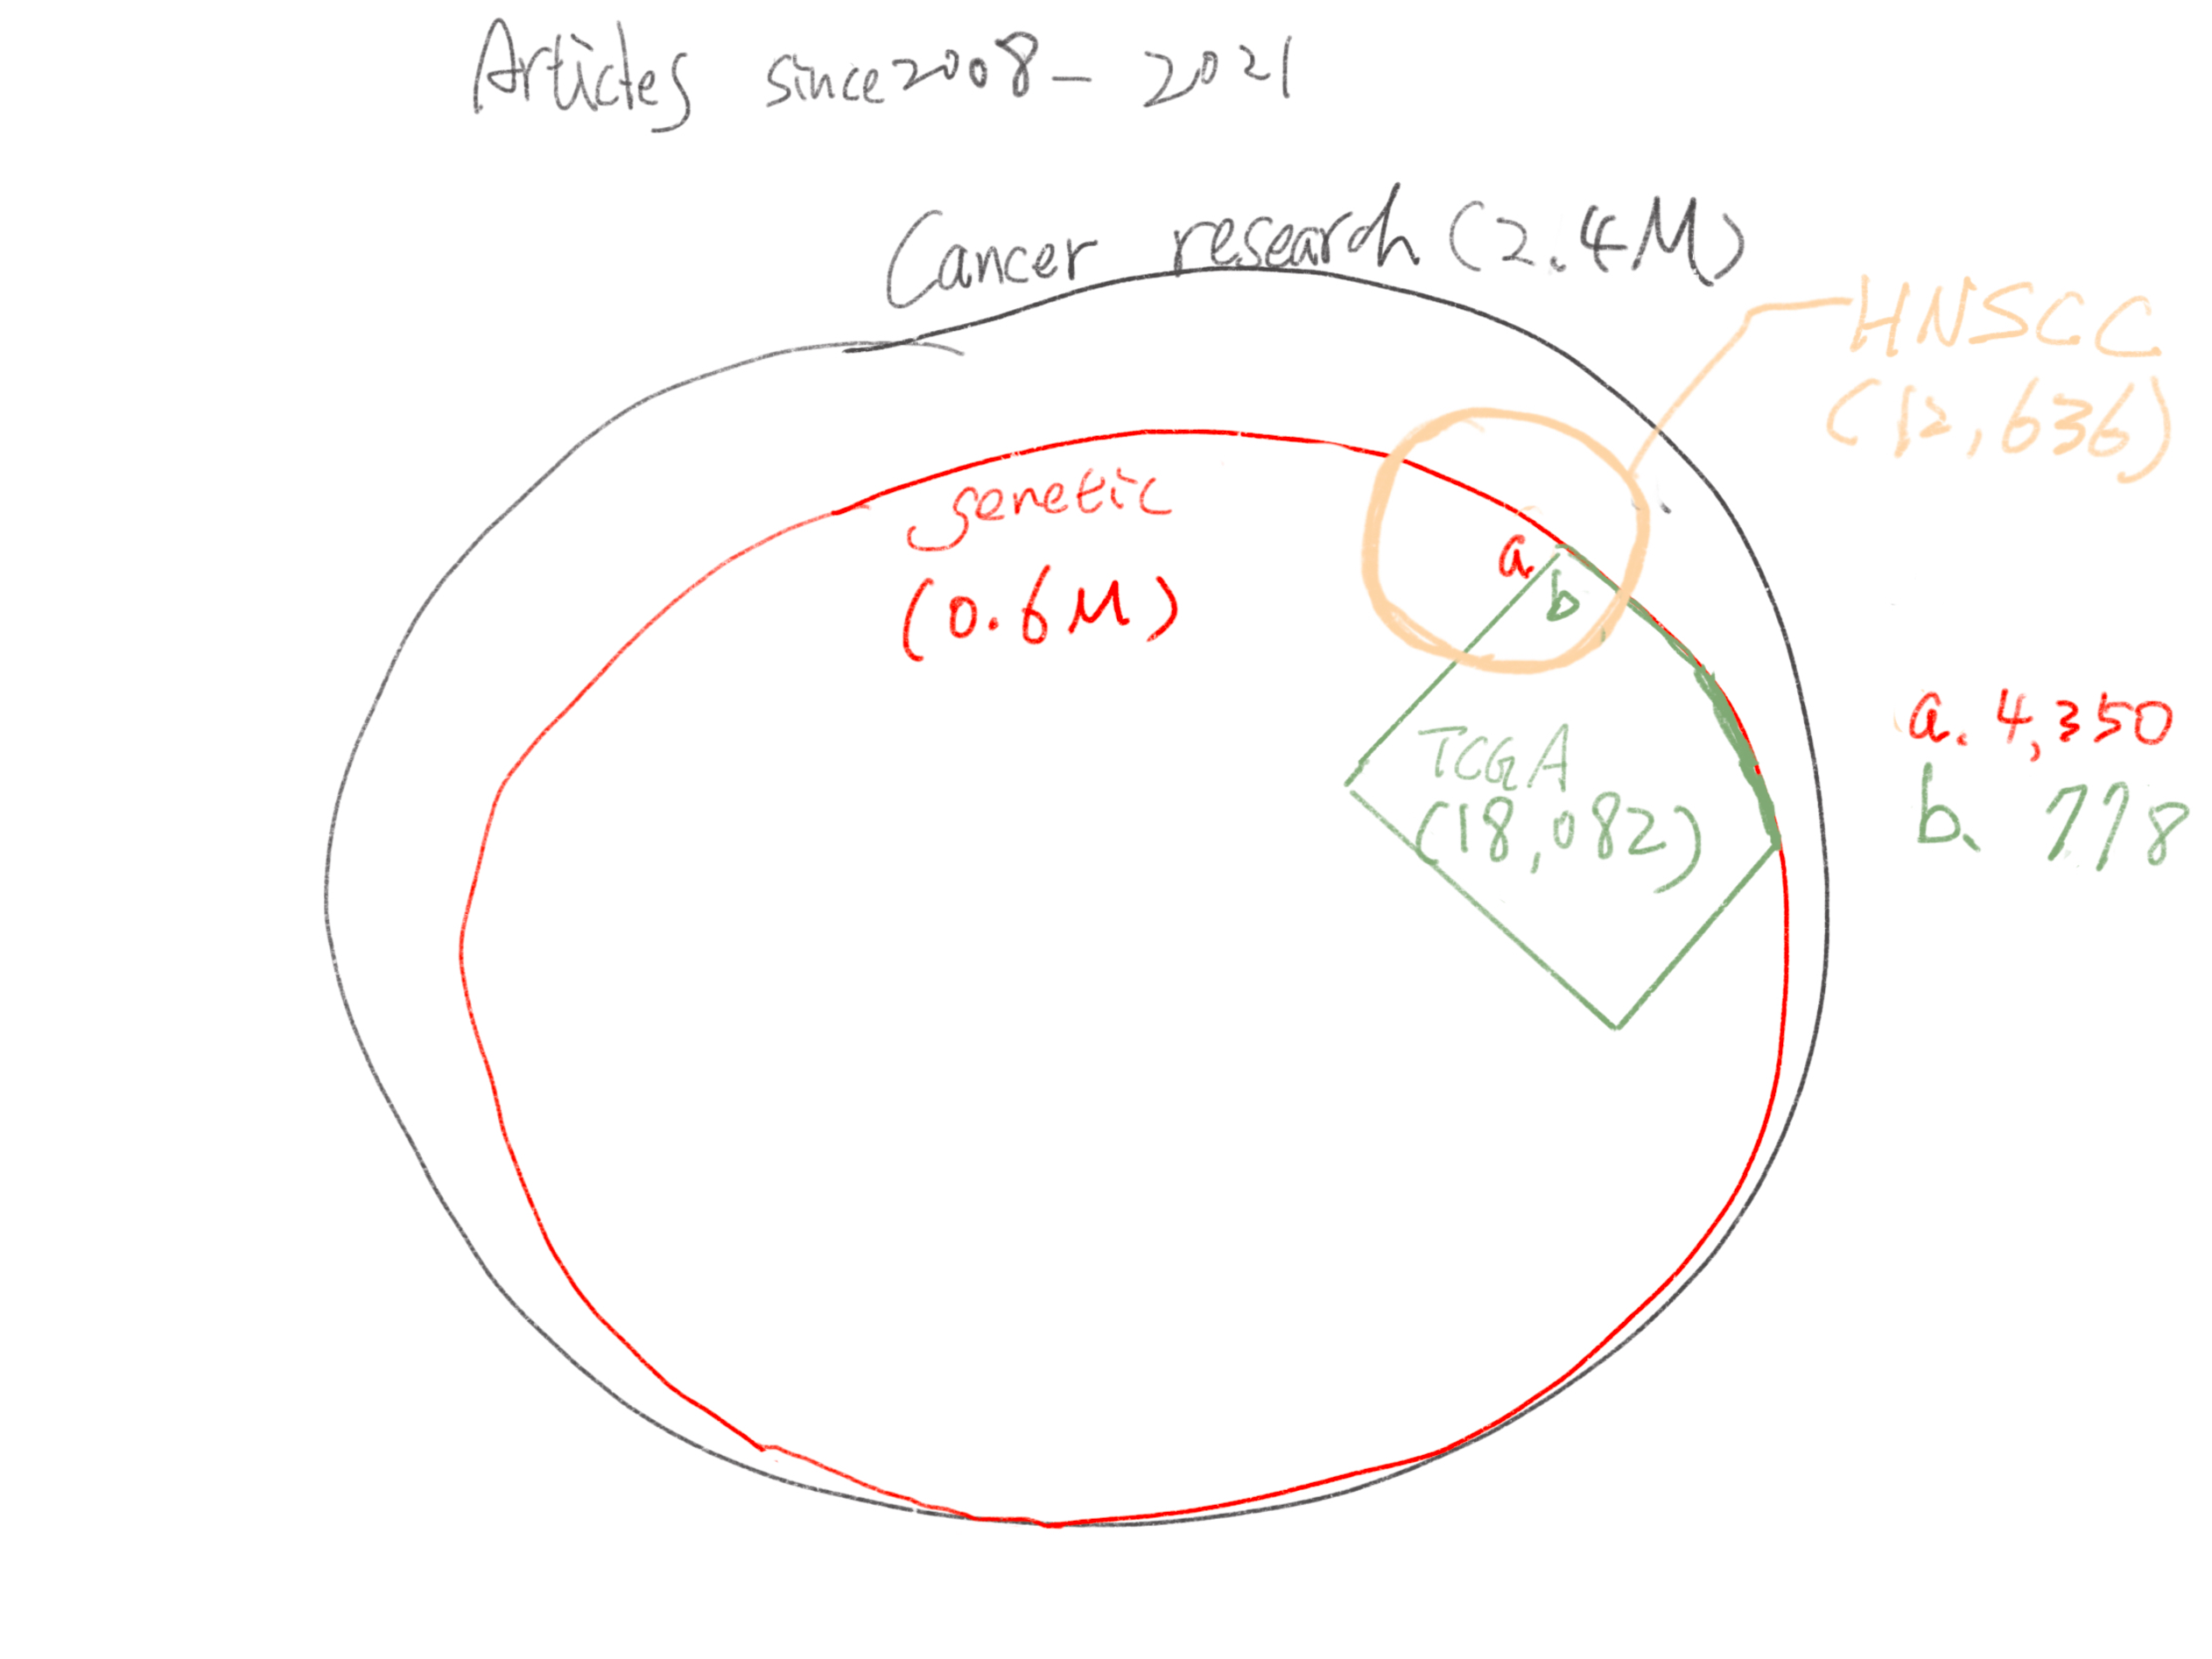
\includegraphics[width=14cm]{Answer_2-1.pdf}
\caption{Cancer research articles published from 2008 to 2021. Total: 2.4 million; genetic related: 0.6 million; HNSCC research: 12,636.}
\label{figure:fig_embase}
\end{figure}
\clearpage
%778/4350 = 17.9\% using TCGA data
%There is 374 genes in the oral cancer gene database of Indian HNSCC; http://www.bioinformation.net/006/97320630006169.pdf
%http://www.actrec.gov.in/OCDB/index.htm

Although other databases carrying HNSCC genomics and clinical data we found, such as MSKCC (151 cases), Broad (74 cases), Johns Hopkins (32 cases), MD Anderson (40 cases), and NCBI Gene Expression Omnibus (GEO) datasets (e.x. GSE2837, 40 cases; GSE6631, 22 cases; GSE31056, 23 cases)\cite{Cerami2012b}\cite{Gao2013a}. However, the MSKCC, Broad, and Johns Hopkins databases were processed through whole-exome sequencing instead of whole-genome sequencing in the TCGA database.

There is several useful web-tools for survival analysis, such as cBioportal\cite{Cerami2012b}\cite{Gao2013a}, KM-Plotter\cite{Gyorffy2010},  SurvExpress\cite{Aguirre-Gamboa2013}, UALCAN (available at http://ualcan\\.path.uab.edu/)\cite{Chandrashekar2017a} and Gene Expression Profiling Interactive Analysis (GEPIA, GEPIA2)\cite{Tang2019}. According to the citing articles\cite{Wu2020} and their online documents, the back-end databases of those web-tools were collected from TCGA, the European Genome-phenome Archive (EGA)\cite{Lappalainen2015} and NCBI GEO datasets (available at https://www.ncbi.nlm.nih.gov/gds). Furthermore, almost all of their survival data came from the TCGA database.
%GEO (few survival features, less than 100 participate in each GSE dataset)
%GSE31056, GSE2837 (Prognoscan)
%there is survival feature: A total of 44 patients (22 HNSCC samples and 22 normal samples) were obtained from GSE6631
%有文章為證1. Lawrence, M. S. et al. Comprehensive genomic characterization of head and neck squamous cell carcinomas. Nature 517, 576–582 (2015).\cite{Lawrence2015a}
%datasets for each cancer type that include exactly the same prediction and outcome variables and consider comparable target populations. Currently, such data is simply not available.

%The Dickkopf1 (DKK1) gene encodes a protein that was mainly involved in Wnt and other signaling pathways.
%Inhibition of DKK1 in Hep-2 cells reduces their proliferation, colony formation, cell migration, and invasion in vitro\cite{Shi2014}.
%Pang et al\cite{Pang2018} demonstrated that upregulation of DKK1 in SBC-3 cells (human small cell lung cancer) enhanced their proliferation, colony formation, cell migration, and invasion in vitro, as well as bone metastasis in vivo. 
%Increased DKK1 levels in HNSCC tissues correlated with elevated VEGF-C and beta-catenin\cite{Shi2014}.
%DKK1 expression was significantly associated with smoking, alcohol abuse, sex, human papillomavirus status\cite{Chakraborty2020}, tumor site, tumor invasion, and pathologic stage in HNSCC patients.\cite{Gao2018}.
%The mRNA expression of DKK1 and DKK3 was elevated in human papillomavirus (HPV)-negative HNSCC\cite{Hu2020}.

For example, Wei et al.\cite{Wei2020} conducted the analysis of the prognostic value of DKK1 expression in human cancers based on bioinformatics tools, including UALCAN, GEPIA2 (dataset from TCGA)\cite{Tang2019}, and DriverDBv3 databases.
%using http://gepia2.cancer-pku.cn/detail.php?gene=DKK1 => \cite{Tang2019}
%GEPIA is a web-based tool that plots expression profiles of given genes (dataset from TCGA database)
They has suggested that overexpression of DKK1 indicates adverse OS in bladder urothelial carcinoma (BLCA)\cite{Wei2020}, HNSCC\cite{Chakraborty2020}\cite{Hu2020}\cite{Wei2020}, and pancreatic adenocarcinoma (PAAD)\cite{Wei2020}. %Moreover, DKK1 is increased in HPV\+ HNSCC leading to the worst prognosis of the patients. 
%\cite{Shi2014}\cite{Gao2018}\cite{Chakraborty2020}(non-TCGA)\cite{Hu2020}\cite{Wei2020}


Conclusion: TCGA database is representative of HNSCC.


\begin{figure}
\raggedleft
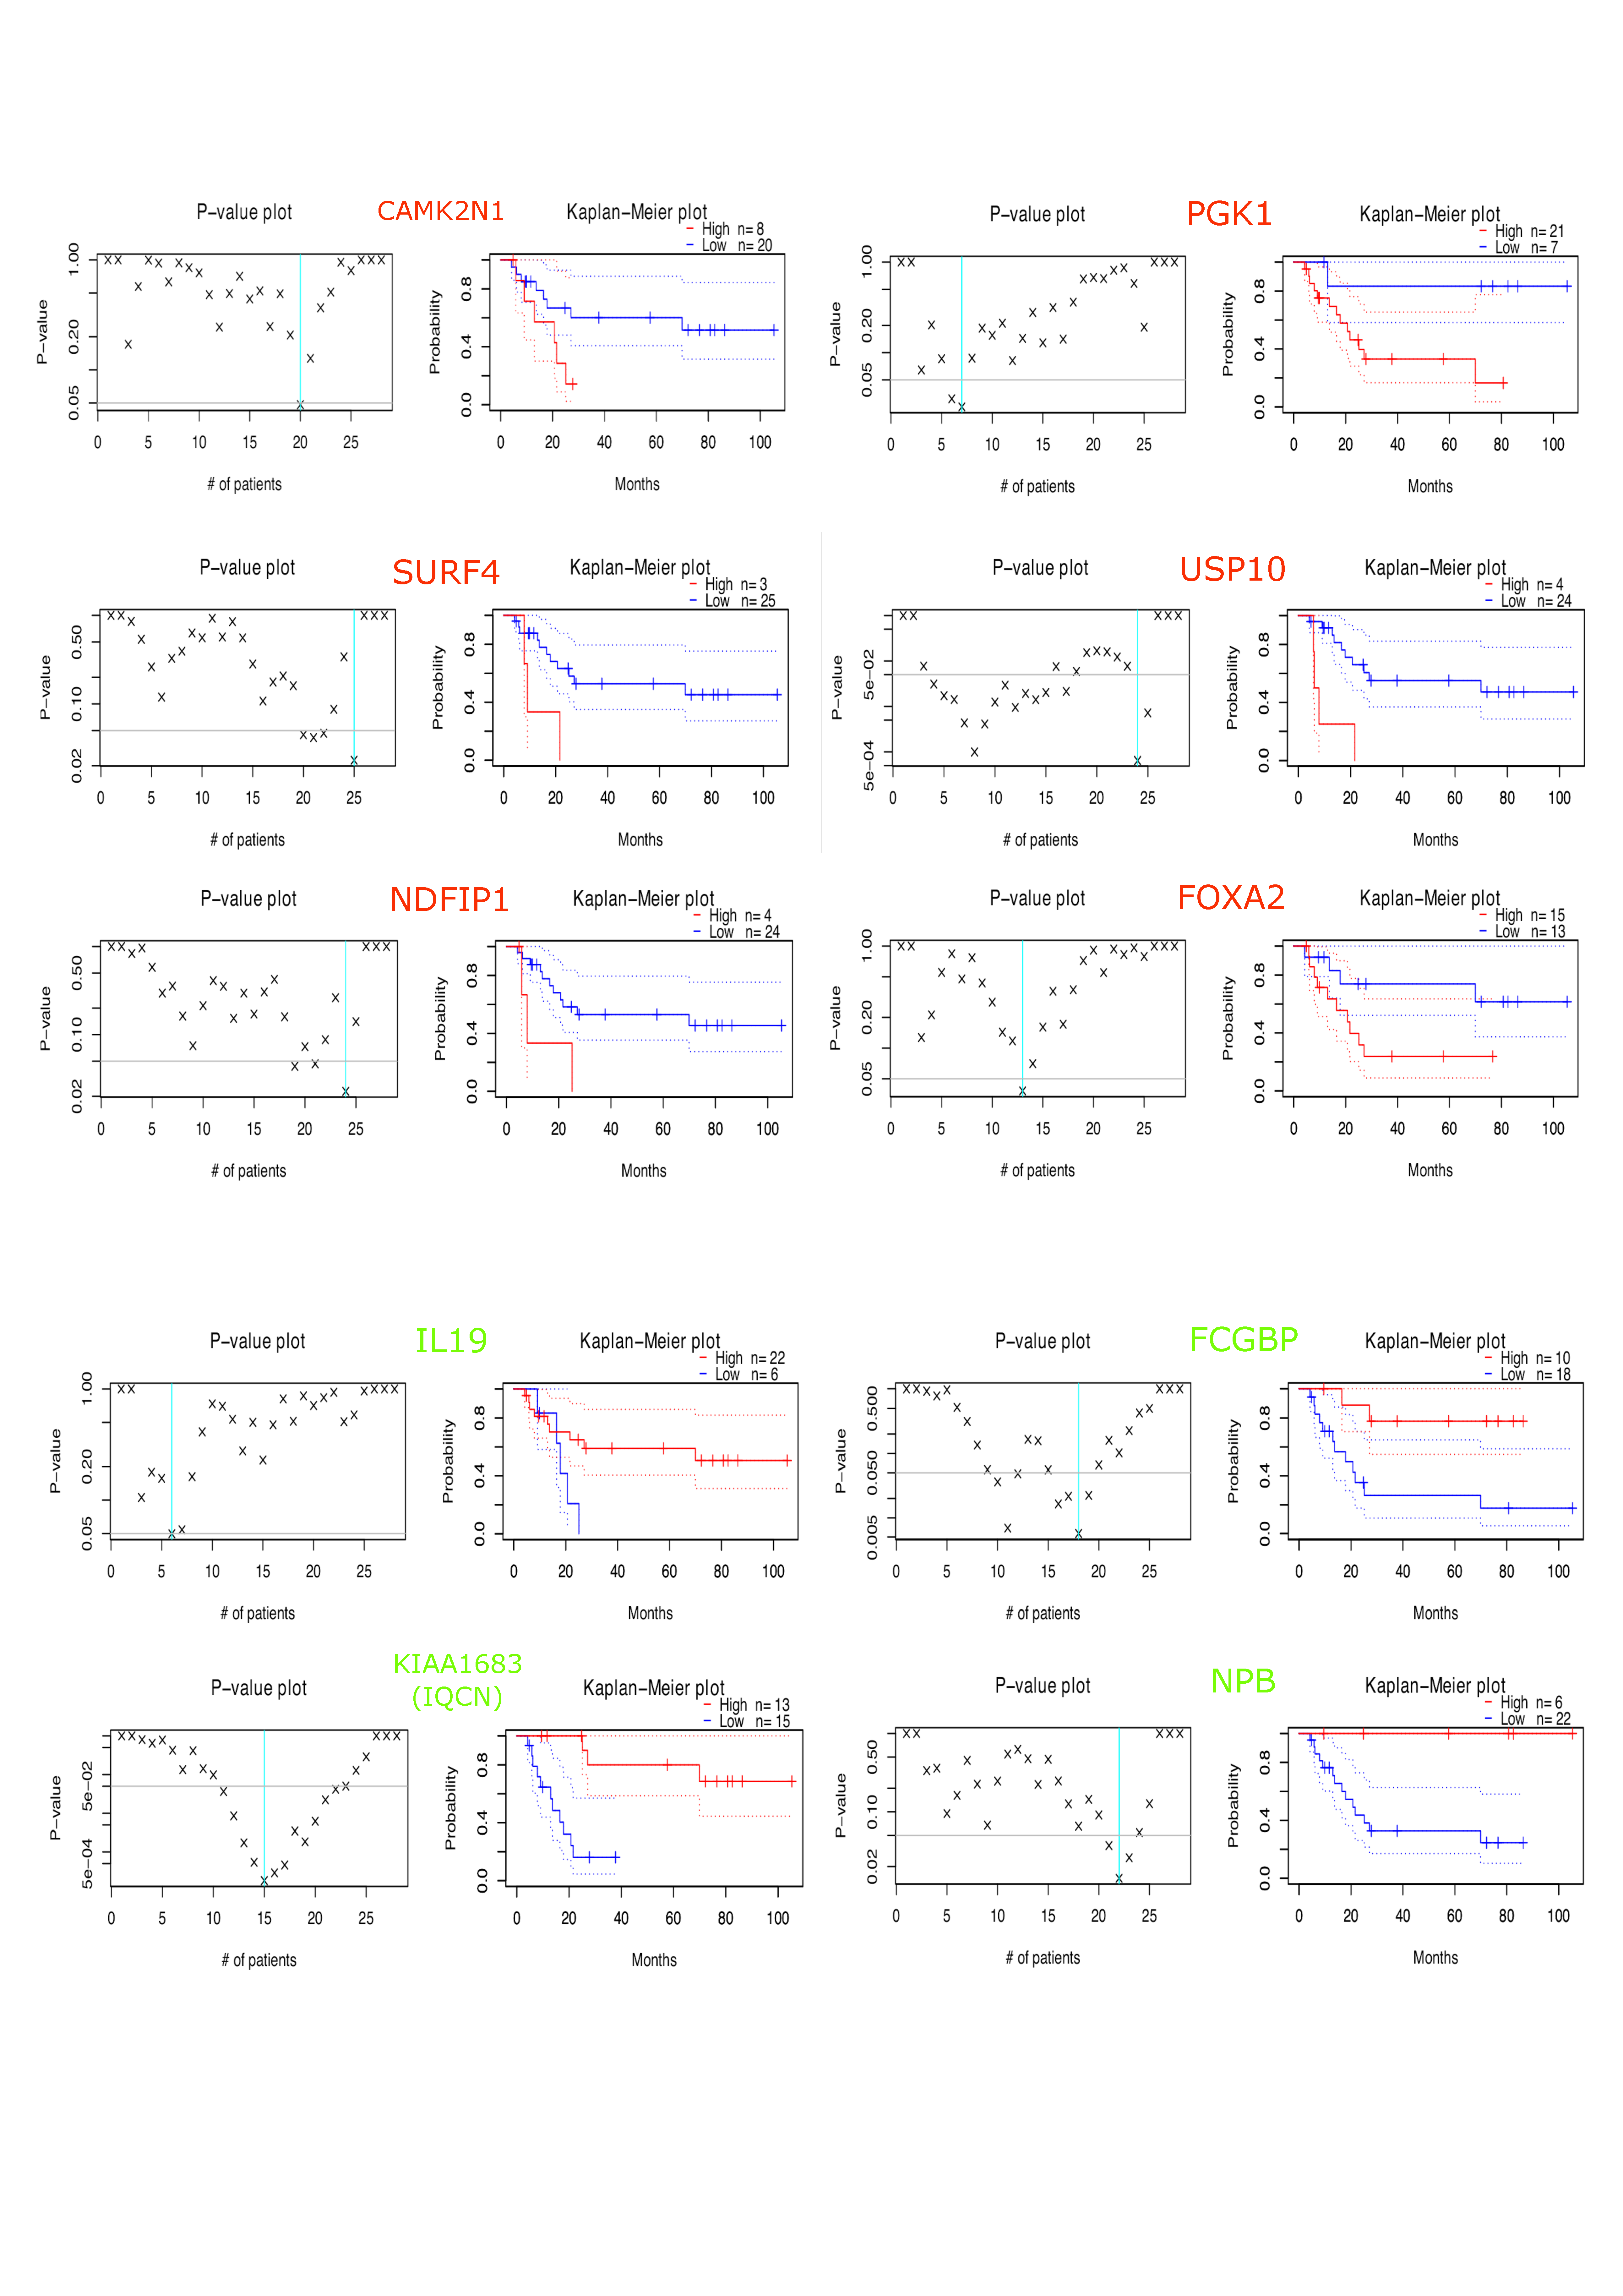
\includegraphics[width=14cm]{Answer_2-2.pdf}
\caption{GSE2837 query results from PrognoScan: Kaplan-Meier plots of 10 genes (the cutoff of \textcolor{red}{high risk} and \textcolor{blue}{low risk} groups, which is derived from cumulative P-value plots). The poor prognostic genes are marked as \textcolor{red}{red}; the better prognostic genes are marked as \textcolor{green}{green}.}
\label{figure:fig_GSE2837}
\end{figure}
\clearpage